\chapter{Mathematical Morphology}
\label{chpt:morphology}

This chapter introduces the notion of mathematical morphology, reflects on its
formalism and details the special case of morphological area opening. We will
take a look at use cases and show the effects of area opening on 2D images. The
chapter concludes with the introduction of the algorithm, which is the basis for
the algorithms developed in this thesis.

Sections~\ref{sec:morphology-area-opening} and \ref{sec:morphology-examples} are
based on a previous project I conducted \cite{Biermann2013Morphological}. The
contents are corrected and cut down to the most relevant parts, for brevity.

\section{Morphological Area Opening}
\label{sec:morphology-area-opening}

This section briefly outlines the formalism of morphological area opening. I
will not go into the details of lattice theory and the foundations of
mathematical morphology. A good reference point for the interested reader is
\emph{An overview of morphological filtering} by \citet{Serra1992Overview}.

Mathematical morphology is, intuitively speaking, the formal study of
shapes. Morphological filters operate on partially ordered sets. Therefore,
morphology only applies to single-channel images, as their elements
(i.e.~pixels) can be ordered by their height (i.e.~gray-scale value)
\cite{Serra1992Overview}. While morphological filtering can also be performed on
binary images, I will omit this case. Computing morphological area openings on
binary images is trivial and reduces to flat component labeling.

Two elementary operations in mathematical morphology are \emph{dilation},
denoted $\delta$, and \emph{erosion}, denoted $\epsilon$, which are mathematical
duals. They are digitally implemented using a structuring element, for example a
disk, a square or a hexagon. Intuitively, erosion extends dark components of an
image, by moving the structuring element around their outer borders. Dilation
does the opposite, narrowing dark elements, by moving the structuring element on
the inner border of the component. The concatenation of both, $\gamma = \epsilon
\circ \delta$, produces the morphological opening of an image. Closing, the
respective dual, is defined as $\varphi = \delta \circ \epsilon$
\cite{Serra1992Overview}. As already pointed out in
chapter~\ref{chpt:introduction}, we will for the remainder only focus on
morphological openings, since area opening and closing are mathematical duals:
computing area opening on an inverted image and inverting the result again,
corresponds to computing area closing \cite{Wilkinson2000Fast}.

Computing the morphological opening of an image $I$, for a structuring element
$S$, removes all bright components from $I$, that do \emph{not} resemble the
shape of $S$ \cite{Serra1992Overview}. This essentially means that, in order to
separate information from the image (i.e. to perform segmentation), we are
required to provide concrete, a priori, non-parametric knowledge
\cite{Vincent1994Morphological}, which sometimes is not available or not
applicable. To work around this problem, a union of multiple openings with
different structuring elements can be constructed, at the cost of filtering an
image repeatedly.

To provide more general means of filtering connected components from an image,
\citet{Vincent1994Morphological} introduced \emph{morphological area opening},
denoted as $\gamma^a_{\lambda}$. In contrast to classical morphological opening,
area opening is performed with a parameter of \emph{area}, or size, called
$\lambda$. One can see area opening as classical morphological opening with a
dynamically shaped structuring element, that adjusts to the structure of the
image and grows up to a certain size. All bright components of an image of size
less than $\lambda$ are removed in its area opening
\cite{Vincent1994Morphological}. Section~\ref{sec:morphology-examples} details
the effects of morphological area opening.

Let an image be represented by a function $f: I \rightarrow \mathbb{R}^*, I
\subset \mathbb{R}^2$. Let, moreover, $T_h(x) \subseteq I, x \in I$ be the
connected component to which $x$ belongs at some gray-value threshold level
$h$. Also, let $\left\vert{}\right\vert$ denote set cardinality. Then, area
opening is defined by \cite{Vincent1994Morphological}:

\begin{equation}
  \gamma^a_{\lambda}(f)(x) = sup\{h \leq f(x) \vert ~ \left\vert{T_h(x)}\right\vert \geq \lambda \}
\end{equation}

This is essentially incremental region-growing for each gray-level threshold of
the input image \cite{Vincent1994Morphological}. This formalism can directly be
projected onto code, resulting in very poor performance, however. A number of
more efficient algorithms have been conceived, which are outlined in the
following section~\ref{sec:morphology-algorithm}.

\section{Usage Example}
\label{sec:morphology-examples}

Typically, area opening is used to either remove unwanted elements, like noise,
from an image, or to identify objects in a scene. Vincent originally proposed to
use area opening to identify micro-aneurysms in images of eye blood-vessels
\cite{Vincent1994Morphological}. One would first compute the area opening of the
image for some $\lambda$, which corresponds to the expected size of aneurysms in
pixels. To identify the location of the aneurysms, it is enough to compute the
pixel-wise difference between the original image and its area opening.

This approach can be used in many different settings. Morphological area opening
has been used in literature for the segmentation of red blood cells in the case
of automated Malaria diagnosis \cite{MohanaRao2001Areagranulometry,
  Tek2010Parasite}. In figure~\ref{fig:morphology-examples-malaria-orig}, we can
see an image of human red blood cells ($800 \times 600$ pixels), infected with
Malaria parasites. The successive images,
\ref{fig:morphology-examples-malaria-1500} through
\ref{fig:morphology-examples-malaria-4500}, show the area closing of the source
image for increasing values of $\lambda$ in pixels. We use area closing here,
because the blood cells are darker than the background. Alternatively, one can
simply compute the negative of the image before and after opening it
\cite{Wilkinson2000Fast}. The bigger $\lambda$ gets, the more cells are removed
from the image, while the background remains unmodified. By those means, we are
able to compute an approximation of the background model, which is helpful for
separating the single blood cells from the image background.

\begin{figure}
  \centering

  \makebox[\textwidth][c]{

    \begin{subfigure}{0.25\textwidth}
      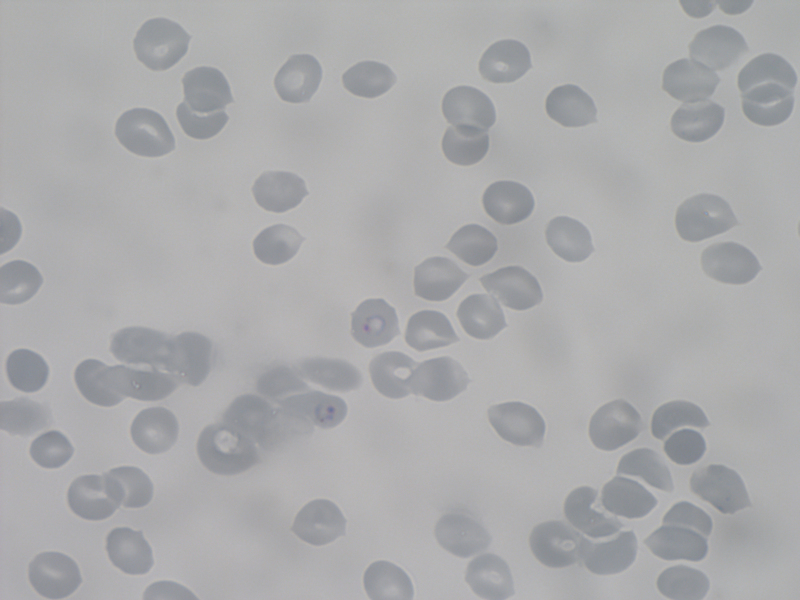
\includegraphics[width=\textwidth]{../data/natural001.jpg}
      \caption{Original image}
      \label{fig:morphology-examples-malaria-orig}
    \end{subfigure}

    \begin{subfigure}{0.25\textwidth}
      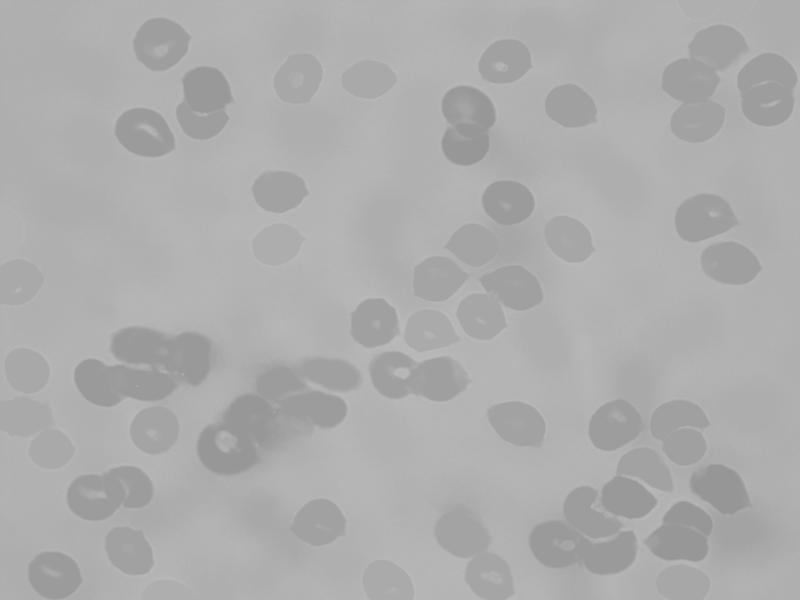
\includegraphics[width=\textwidth]{images/area-closing-1500.jpg}
      \caption{$\lambda = 1500$}
      \label{fig:morphology-examples-malaria-1500}
    \end{subfigure}

    \begin{subfigure}{0.25\textwidth}
      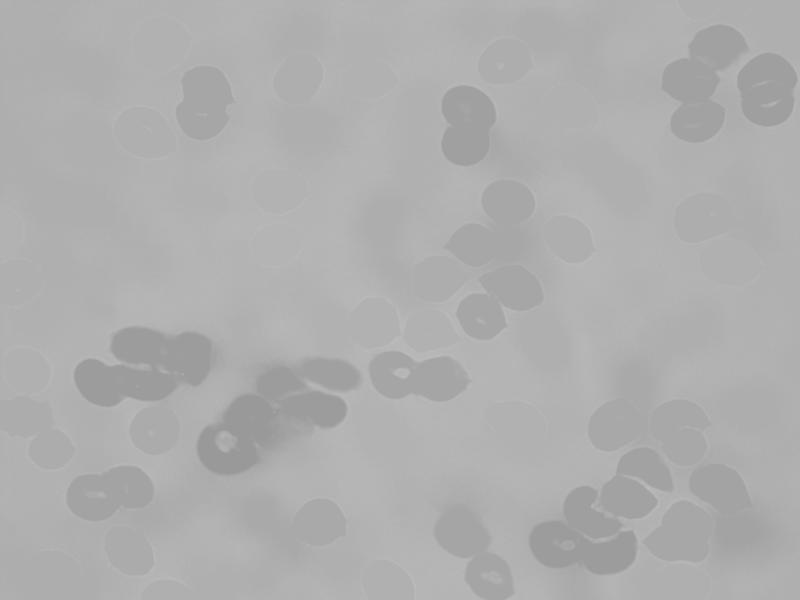
\includegraphics[width=\textwidth]{images/area-closing-3000.jpg}
      \caption{$\lambda = 3000$}
      \label{fig:morphology-examples-malaria-3000}
    \end{subfigure}

    \begin{subfigure}{0.25\textwidth}
      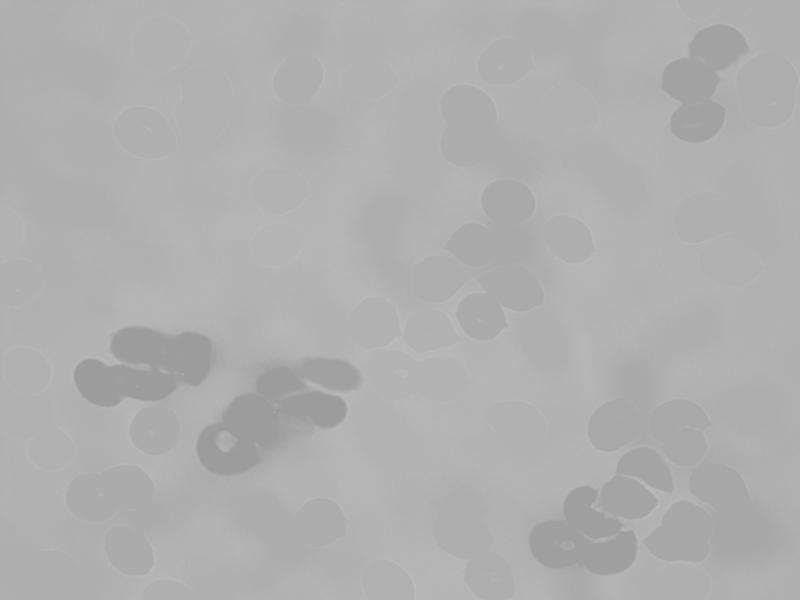
\includegraphics[width=\textwidth]{images/area-closing-4500.jpg}
      \caption{$\lambda = 4500$}
      \label{fig:morphology-examples-malaria-4500}
    \end{subfigure}

  } % makebox

  \caption[Area closing (dual to area opening) for increasing values of
  $\lambda$.]{Area closing (dual to area opening) for increasing values of
    $\lambda$ on an image of red blood cells infected with Malaria ($800 \times
    600$ pixels). The larger $\lambda$ becomes, the more blood cells are
    filtered from the image.}
  \label{fig:morphology-examples-malaria}
\end{figure}

\section{Algorithms}
\label{sec:morphology-algorithm}

There exist three well studied algorithms for computing morphological area
opening. Vincent \cite{Vincent1994Morphological} originally described an
algorithm based on gray-scale reconstruction, that requires multiple scans of
the input image using priority queues.

A faster algorithm based on Max-Trees was proposed by
\citet{Salembier1998Antiextensive}. Max-Trees are rooted trees where each node
represents a connected, flat level component. Regional maxima are represented by
the leaves of the tree. Filtering is then only a matter of removing all nodes of
size less than $\lambda$. It is easily generalized for a wide range of
morphological filters, such as morphological thinnings
\cite{Breen1996Attribute}. \citet{Wilkinson2008Concurrent} developed a parallel
version of this algorithm. They split the input image in $n \geq t$ sub-images,
where $t$ is the number of available hardware threads. For each sub-image, a
Max-Tree is computed in parallel. In a subsequent, sequential routine, the
independently computed trees are merged and, finally, filtered.

\citet{Meijster2002Comparison} proposed a region growing algorithm to compute
morphological area openings based on Tarjan's union-find data structure
\cite{Tarjan1983Data}. They extended their algorithm to compute the size
distribution of elements on an image, called area granulometry
\cite{Meijster2001Fast}. The parallel algorithms developed in this thesis extend
this union-find based algorithm. The remainder of this section contains a
detailed description of the algorithm by \citet{Meijster2002Comparison}.

A pixel $i$ at the coordinates $(x, y)$ is represented as single integer value,
computed by $i = w \cdot y + x$ where $w$ is the width of the input image
\cite{Meijster2002Comparison}. Connected components are represented by a
disjoint-tree structure, where the root of each tree is represented by the last
visited pixel. An input image is represented using two arrays:

\begin{itemize}
\item \inlinecode{value}, which stores an integer representation of the
  gray-scale value of each pixel. During the main loop, this array is read only.

\item \inlinecode{parent}, which represents the index of the parent pixel in the
  union-find data structure if \inlinecode{parent[i]} $\geq 0$, or the size of
  the tree of which \inlinecode{i} is the root, if \inlinecode{parent[i]} $< 0$.
\end{itemize}

\begin{figure}
  \centering
  \lstinputlisting[widthgobble=1*0,linerange={union0-union1}]{../parallel-morphology/src/dk/itu/parallel/morphology/unionfind/SequentialUnionFind.java}
  \caption{The \inlinecode{union} function for conditional region growing.}
  \label{fig:morphology-algorithm-union}
\end{figure}

\begin{figure}
  \centering
  \lstinputlisting[widthgobble=1*0,linerange={uniteNeighbors0-uniteNeighbors1}]{../parallel-morphology/src/dk/itu/parallel/morphology/filter/base/Filter.java}
  \caption{The \inlinecode{uniteNeighbors} function that calls \inlinecode{union}.}
  \label{fig:morphology-algorithm-uniteNeighbors}
\end{figure}

For simplicity, both arrays are also accessible through equally named
functions. Using negative integers to represent tree size instead of parent
index, allows us to minimize memory usage \cite{Meijster2002Comparison}. We are
furthermore given the following functions:

\begin{itemize}
\item \inlinecode{union(n, c, lambda)} unites the trees containing the pixels at
  \inlinecode{n} and \inlinecode{c} for a given size parameter
  \inlinecode{lambda} (see figure~\ref{fig:morphology-algorithm-union})
  \cite{Meijster2002Comparison}.

\item \inlinecode{find(x)} returns the root index of the tree containing the
  pixel at \inlinecode{x} and compresses the path between \inlinecode{x} and the
  root \cite{Tarjan1983Data, Meijster2002Comparison}.

\item \inlinecode{neighbors(x)} returns all indices of the pixels adjacent to
  \inlinecode{x}, assuming 8-connectivity.

\item \inlinecode{uniteNeighbors(x, lambda)} unites the pixel at \inlinecode{x}
  with all its valid neighbors.
\end{itemize}

To compute area opening, we must first identify regional maxima on the image
\cite{Vincent1994Morphological}. The algorithm by \citet{Meijster2002Comparison}
does this by sorting image pixels by gray-scale value. The so sorted pixel
indices are stored in an additional array \inlinecode{sorted}. Sorting can be
performed in linear time using counting-sort \cite{Meijster2002Comparison}.

The next step is to let connected components of pixels grow conditionally, if,
after the definition of area opening, neighboring connected components belong to
the same connected component. The function \inlinecode{uniteNeighbors(c, lambda)}
unites a pixel with all its valid neighbors and is shown in detail in
figure~\ref{fig:morphology-algorithm-uniteNeighbors}.

If \inlinecode{c} is at level with \inlinecode{n}, the pixel pair is valid. This
is essentially flat component labeling \cite{Meijster2002Comparison}. Moreover,
a pixel is allowed to join a set ``upwards'' in gray-level hierarchy, so to
unite with a pixel of higher gray-value: this is the first part of growing
connected components. The gray-level sorted pixels are iterated in decreasing
gray-value order. This is the main loop of union-find based area opening
\cite{Meijster2002Comparison}:

\lstinputlisting[linerange={filter0-filter1},frame=L]{../parallel-morphology/src/dk/itu/parallel/morphology/filter/Sequential.java}

However, \inlinecode{union} does not unite disjoint trees
unconditionally. Instead, it allows connected components only to be united, if
either the root of \inlinecode{n} is at level with \inlinecode{c}, or, if the
area of the connected component containing \inlinecode{n}, is less than
\inlinecode{lambda}. If none of these conditions are fulfilled, \inlinecode{c}
is deactivated: its size is simply set to \inlinecode{lambda} and no component
may exceed \inlinecode{lambda}, unless it is a level-component (i.e. all pixels
of the component are at the same gray-level) \cite{Meijster2002Comparison}. If
the trees are united, the last visited pixel \inlinecode{c} becomes the new
root. Thereby, the darkest pixel of the connected component is always the root
of the tree. Building paths in this fashion directly contradicts the idea of
ranking and swapping trees, in order to maintain short paths
\cite{Tarjan1983Data}. \citet{Meijster2002Comparison} leave this contradiction
uncommented.

This algorithm a simplified version of the one given by
\citet{Meijster2002Comparison}. Their original algorithm performs on-the-fly
initialization of the disjoint set structure, which is possible because, in a
sequential program, counting sort is stable w.r.t. the prior order of
elements. This implies that it is enough to find the root of \inlinecode{n}
during \inlinecode{union}, as \inlinecode{c} has not yet been initialized as a
singleton. Every pixel's singleton is initialized when
\inlinecode{uniteNeighbors} is called on it. The original condition (compared to
figure~\ref{fig:morphology-algorithm-uniteNeighbors}), to determine whether a
pixel should be united with its neighbors, is \cite{Meijster2002Comparison}:

\begin{lstlisting}[style=inline]
  value(c) <= value(n) || (value(c) == value(n) && n < c)
\end{lstlisting}

This structure gives the linear code advantages, which are hard to achieve in
parallel algorithms. For the remainder of this thesis, I will only consider the
simplified version of the algorithm, so that the order of level pixels is
neglected. The detailed implementation of the simplified \inlinecode{union}
algorithm is depicted in figure~\ref{fig:morphology-algorithm-union}.

Always making the last visited, and thereby darkest, pixel root of its set
enables us to use a simple resolving step, that finalizes the algorithm. The
list of sorted pixels is iterated in reverse order and each pixel is assigned
the gray-scale value of its root. Thereby, we filter regional maxima from the
image \cite{Meijster2002Comparison}:

\begin{lstlisting}[frame=L]
    // Resolve gray-values.
    for (final int s : sorted) {
      if (parent(s) > 0) // Only update child-nodes.
        image().pixel[s] = value(find(s));
    }
\end{lstlisting}

This final step will not be part of further discussion, as it can easily be
parallelized. We are mainly interested in building the correct union-find
structure to represent connected components.

%%% Local Variables:
%%% mode: latex
%%% TeX-master: "main"
%%% End:
